\let\negmedspace\undefined
\let\negthickspace\undefined
\documentclass[journal]{IEEEtran}
\usepackage[a5paper, margin=10mm, onecolumn]{geometry}
%\usepackage{lmodern} % Ensure lmodern is loaded for pdflatex
\usepackage{tfrupee} % Include tfrupee package

\setlength{\headheight}{1cm} % Set the height of the header box
\setlength{\headsep}{0mm}     % Set the distance between the header box and the top of the text

\usepackage{gvv-book}
\usepackage{gvv}
\usepackage{cite}
\usepackage{amsmath,amssymb,amsfonts,amsthm}
\usepackage{algorithmic}
\usepackage{graphicx}
\usepackage{textcomp}
\usepackage{xcolor}
\usepackage{txfonts}
\usepackage{listings}
\usepackage{enumitem}
\usepackage{mathtools}
\usepackage{gensymb}
\usepackage{comment}
\usepackage[breaklinks=true]{hyperref}
\usepackage{tkz-euclide} 
\usepackage{listings}
% \usepackage{gvv}                                        
\def\inputGnumericTable{}                                 
\usepackage[latin1]{inputenc}                                
\usepackage{color}                                            
\usepackage{array}                                            
\usepackage{longtable}                                       
\usepackage{calc}                                             
\usepackage{multirow}                                         
\usepackage{hhline}                                           
\usepackage{ifthen}                                           
\usepackage{lscape}
\begin{document}

\bibliographystyle{IEEEtran}
\vspace{3cm}

\title{Ellipse Question}
\author{EE24BTECH11040 - Mandara Hosur}
% \maketitle
% \newpage
% \bigskip
{\let\newpage\relax\maketitle}

\renewcommand{\thefigure}{\theenumi}
\renewcommand{\thetable}{\theenumi}
\setlength{\intextsep}{10pt} % Space between text and floats


\numberwithin{equation}{enumi}
\numberwithin{figure}{enumi}
\renewcommand{\thetable}{\theenumi}

\textbf{Question:}\\
For the differential equation given below, find a particular solution that satisfies y=1 when x=0:
$$\brak{x^3 + x^2 + x + 1}\frac{dy}{dx} = 2x^2 + x$$
\\ \\
\textbf{Solution:} \\
The required particular solution can be found using the method of finite differences. 

\begin{align}
\frac{dy}{dx} = \frac{y(x+h) - y(x)}{h} \\
\implies y(x+h) = y(x) + h\cdot\frac{dy}{dx}
\end{align}

As can be seen from the question above,

\begin{align}
\frac{dy}{dx} = \frac{2x^2 + x}{\brak{x^3 + x^2 + x + 1}} \\
\implies y(x+h) = y(x) + h\cdot\frac{2x^2 + x}{\brak{x^3 + x^2 + x + 1}}
\label{0.4}
\end{align}

Let $x_0 = 0$ and $y_0 = 1$ (as per the given condition) \\
Let some $x_1 = x_0 + h$. Then
\begin{align}
y_1 = y_0 + h\cdot\frac{2x_0^2 + x_0}{\brak{x_0^3 + x_0^2 + x_0 + 1}}
\label{0.5}
\end{align}

Iterating through the above-mentioned process to generate $y_2$, $y_3$, $y_4$ and so on generalises equation \eqref{0.5} to

\begin{align}
y_{n+1} = y_n + h\cdot\frac{2x_n^2 + x_n}{\brak{x_n^3 + x_n^2 + x_n + 1}}
\end{align}

The smaller the value of $h$, the more accurate the curve is. \\

The equation of the curve is found by manual methods is
\begin{align}
y = \frac{1}{4}\ln{\brak{\brak{x+1}^2\brak{x^2+1}^3}} - \frac{1}{2}\tan^{-1}{x} + 1
\end{align}

The curve generated using the method of finite differences for the given question, taking $h=0.1$ and running iterations $100$ times is given below.

\begin{figure}[h]
	\centering
	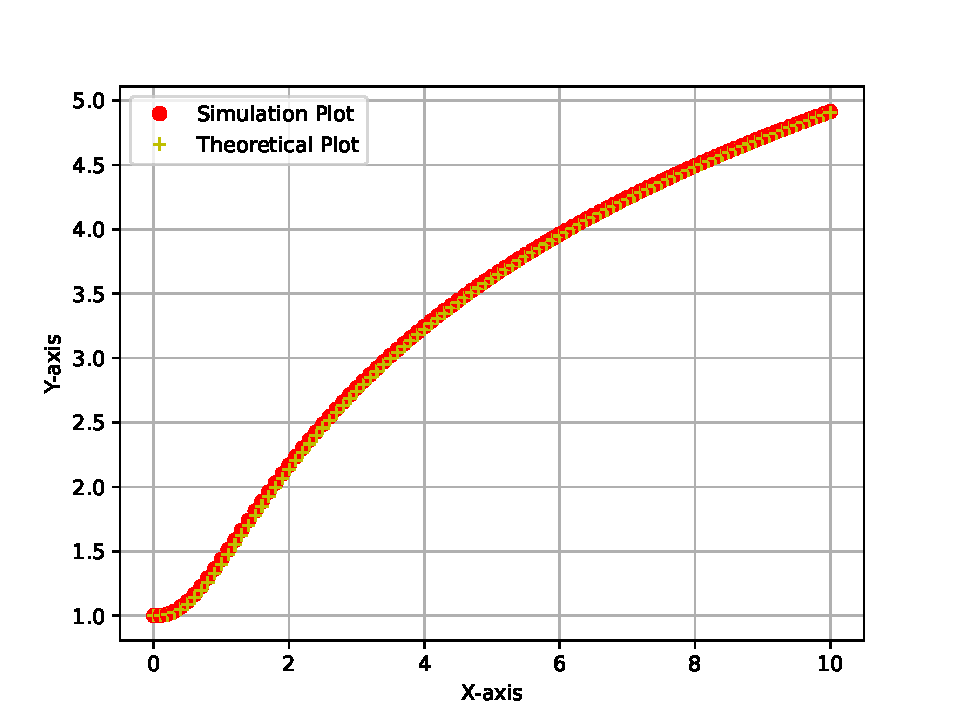
\includegraphics[width=\columnwidth]{figs/fig.pdf}
	\caption{Solution of given DE}
	\label{fig}
\end{figure}

\end{document}
